% Indicate the main file. Must go at the beginning of the file.
% !TEX root = ../main.tex

%----------------------------------------------------------------------------------------
% EINLEITUNG
%----------------------------------------------------------------------------------------


\chapter{Einleitung} % Main chapter title


\label{Chapter1} % Change X to a consecutive number; for referencing this chapter elsewhere, use \ref{ChapterX}

%----------------------------------------------------------------------------------------
% SECTION 1
%----------------------------------------------------------------------------------------

\section{Ausgangslage}
\label{sec:Ausgangslage} 
Code Reviews sind ein wichtiger Bestandteil der modernen Softwareentwicklung. Reviews fördern nicht nur die Qualität des Codes, sondern auch die Zusammenarbeit im Team \parencite{dos_santos_investigating_2018}. In der Praxis werden Code Reviews häufig über Plattformen wie GitHub oder GitLab durchgeführt. Dabei werden auf der Plattform sogenannte Pull Requests / Merge Requests erstellt, welche dann als Grundlage für die Reviews dienen. Die Bezeichnung kann sich von Plattform zu Plattform ändern, beschreibt aber jeweils dasselbe Konzept. \parencite{kansab_analyzing_2025}


Die Analyse der Code-Review-Daten kann wertvolle Informationen über die Zusammenarbeit und den Fortschritt innerhalb eines Softwareprojekts liefern. Eine automatisierte Auswertung bietet die Möglichkeit, Probleme oder Verbesserungsmöglichkeiten zu erkennen. Diese können sowohl auf technischer als auch sozialer Ebene sein. 

An der Zürcher Hochschule für Angewandte Wissenschaften (ZHAW) lernen die Studierenden in Projektmodulen, wie man Projekte erfolgreich durchführt. Für die Zusammenarbeit der Teams wird GitHub eingesetzt. Eine automatisierte Auswertung der Code Reviews kann den Dozierenden helfen, Probleme bei den Studierenden frühzeitig zu erkennen.

Das in der ZHAW entwickelte Tool \textit{GitGauge} ist ein Repository-Mining- und Analyse-Tool, welches aktuell primär für den Einsatz an den Projektmodulen eingesetzt wird. Das Tool wurde im Rahmen einer Mastervertiefungsarbeit von Joel Grand mit Unterstützung des Supervisors Michael Wahler erstellt. GitGauge bietet eine auf \textit{Next.js} basierende Benutzeroberfläche. Der Server wurde in \textit{C\# mit .NET Core } entwickelt. Ziel dieser Arbeit ist es, die Analysen mit diesem Tool durchzuführen und gegebenenfalls, wo nötig, zu erweitern. \parencite{grand_joel_wahler_michael_waspe_lara_stumpf_simon_repo_nodate}

\begin{figure}[htbp]
    \centering
    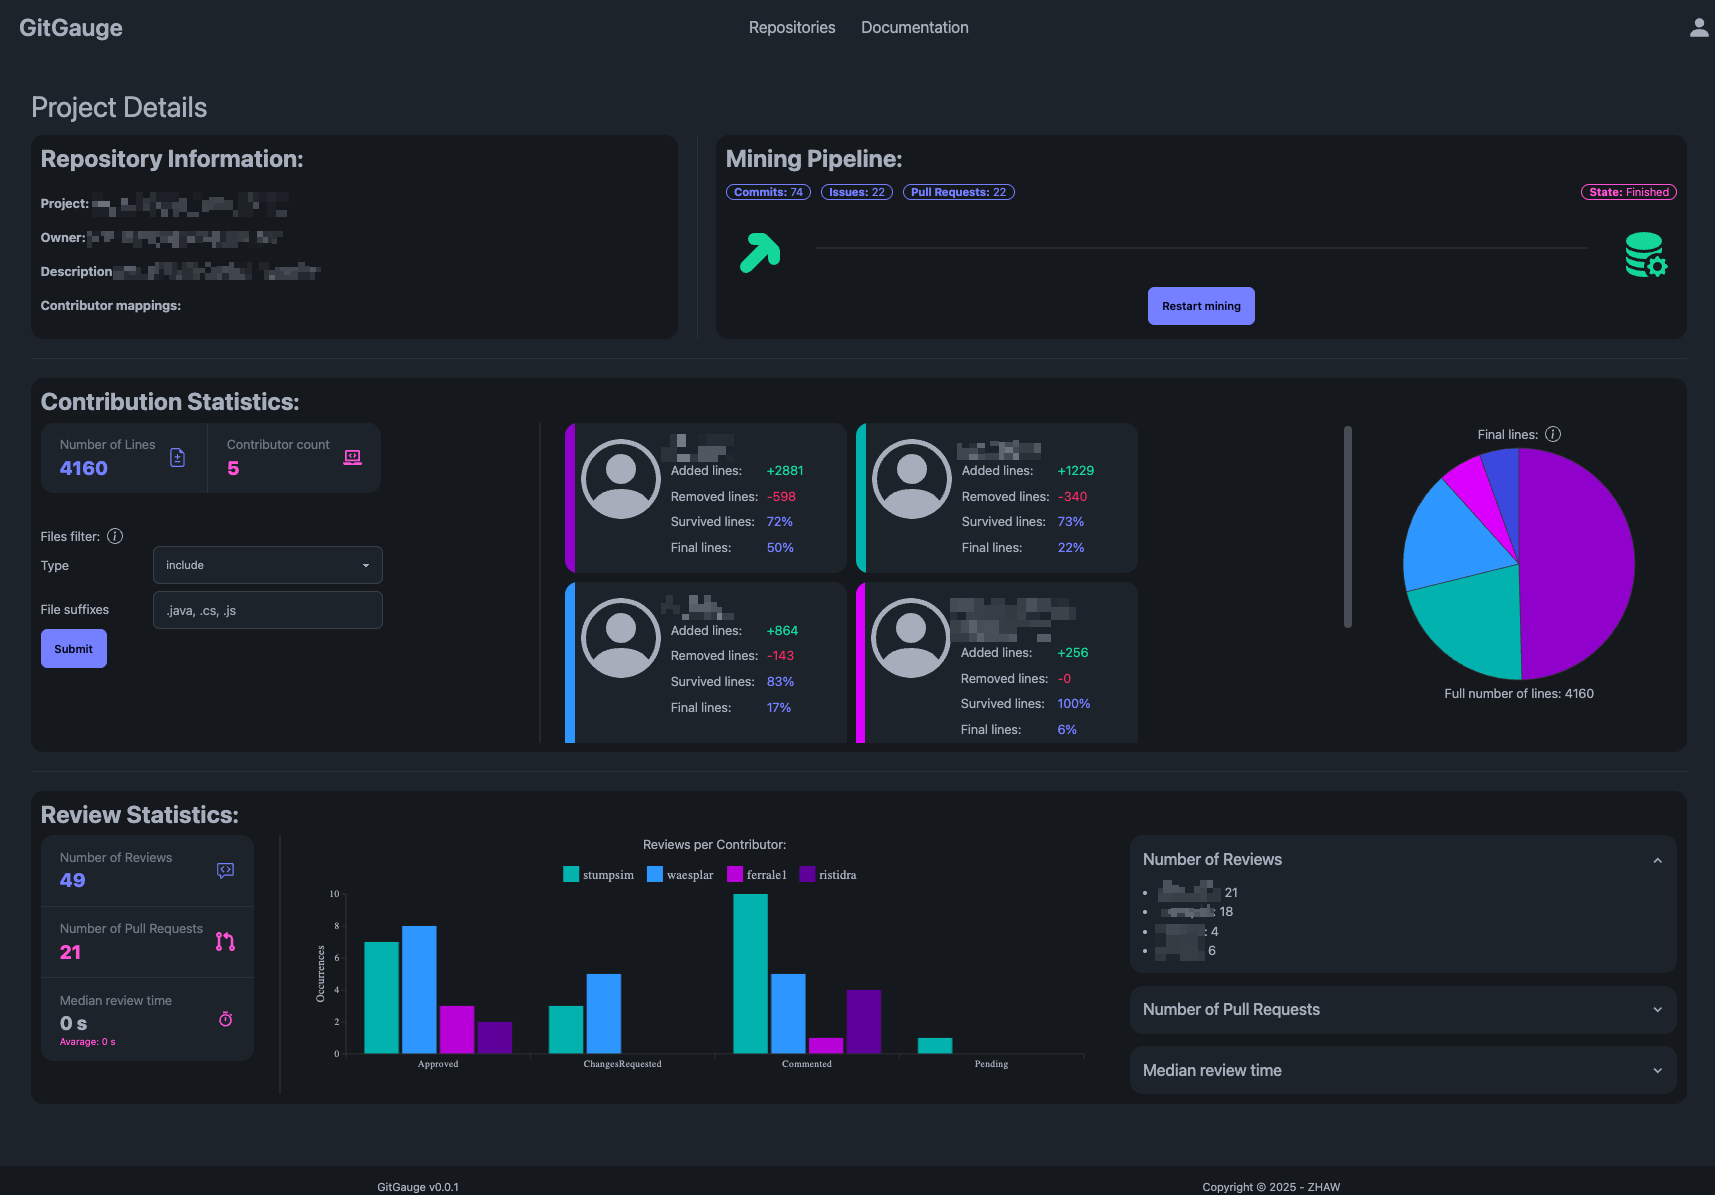
\includegraphics[width=0.8\textwidth]{Figures/giggauge-overview.png}
    \caption{Übersicht eines Projektes in GitGauge}
    \label{fig:gitgauge-project-overview}
\end{figure}

\newpage


\subsection{Vergleichbare Projekte}
Es existieren bereits mehrere Git-Analyse-Tools, die die Untersuchung von Repository-Metriken, insbesondere den Code-Reviews, ermöglichen. 

\textit{Apache Kibble} ist ein OpenSource-Projekt, welches das Minen, Aggregieren und Visualisieren von Softwareprojekten ermöglicht. Viele der bereitgestellten Metriken fokussieren sich jedoch auf die OpenSource-Aspekte eines Projektes, wie etwa die Anzahl Autoren pro Zeitperiode. Ausserdem ist das Projekt nicht besonders aktiv, es wurden lediglich 1 Commit in den letzten 2 Jahren getätigt \parencite{noauthor_apachekibble-1_2025}. Jedoch ist das Projekt gemäss der Apache Webseite noch aktiv \parencite{noauthor_apache_nodate}. Abbildung \autoref{fig:apache-kibble} zeigt einen Auschnitt der offizllen Demo. 
\begin{figure}[htbp]
    \centering
    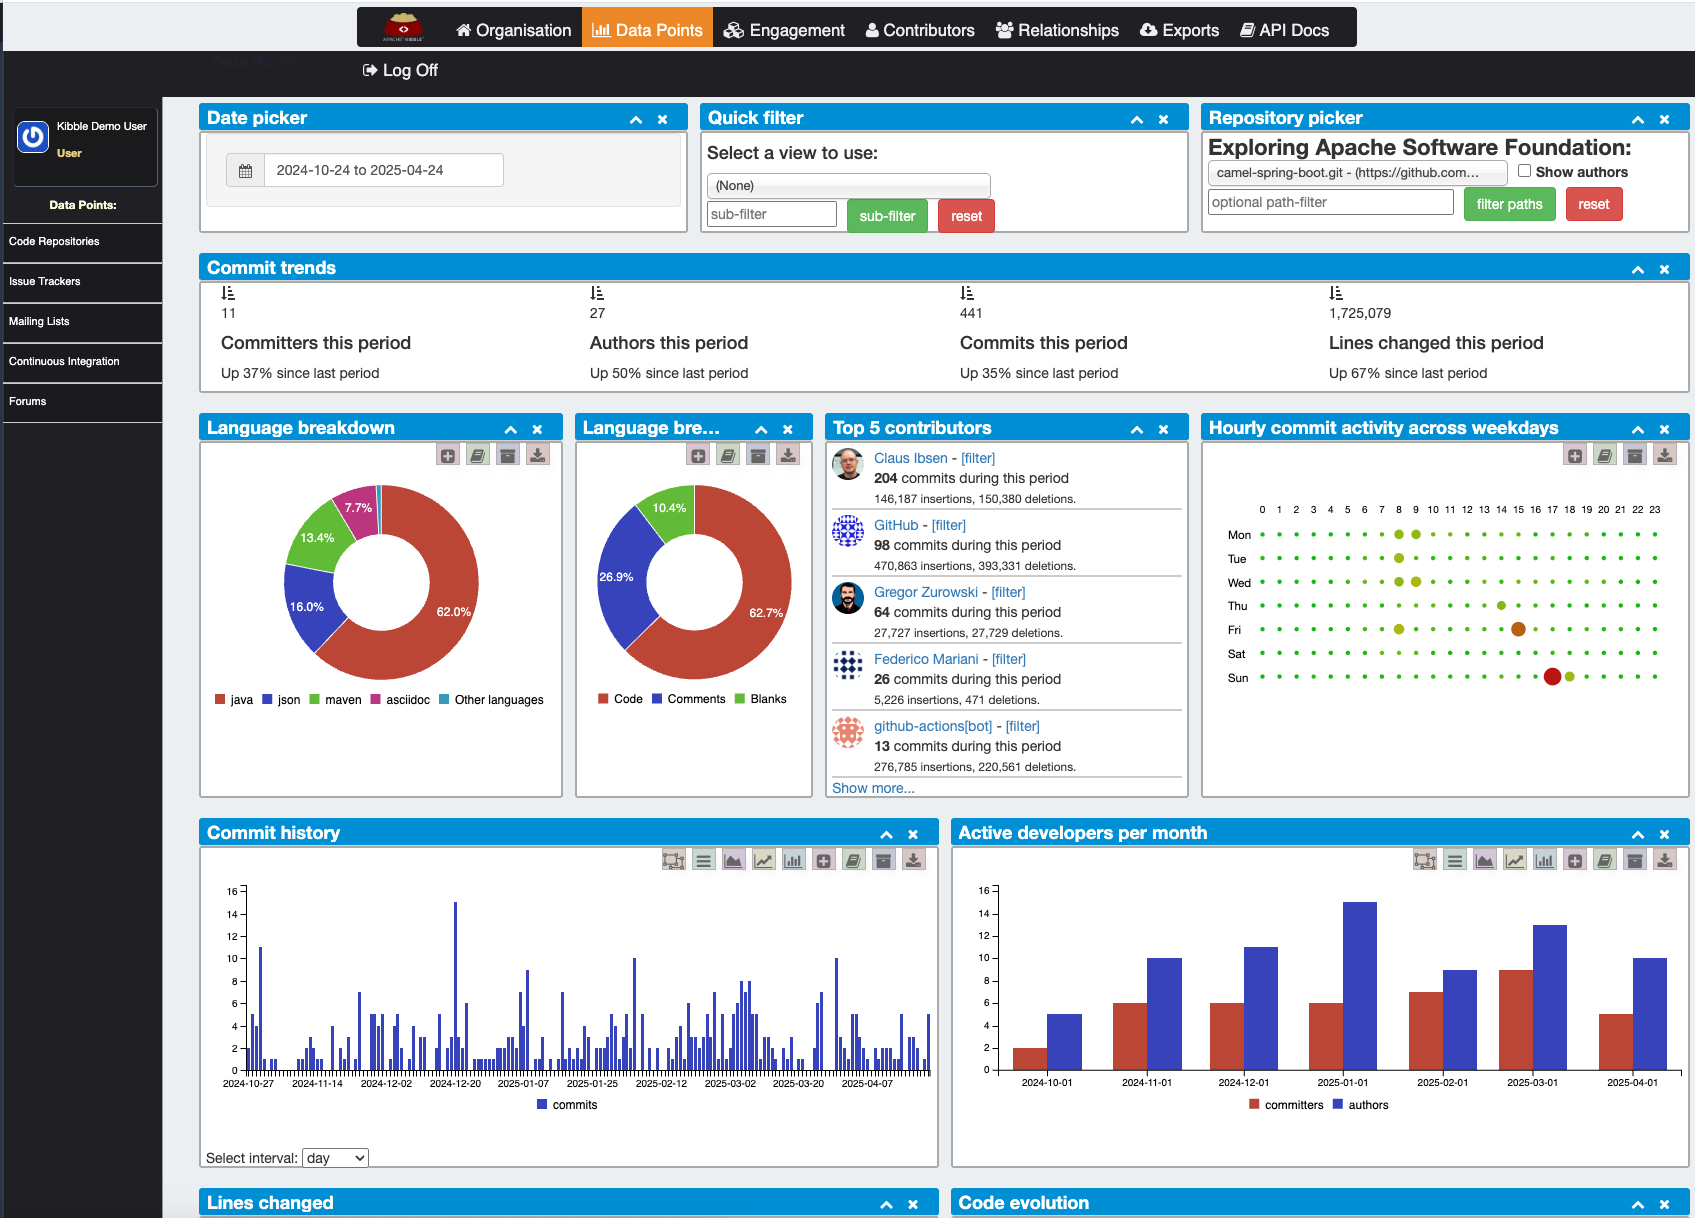
\includegraphics[width=0.8\textwidth]{Figures/apache-kibble.png}
    \caption{Screenshot der Apache Kibble Demo \parencite{noauthor_code_nodate}}
    \label{fig:apache-kibble}
\end{figure}
\newpage
\textit{Augur} ist ein Data Engineering Tool und REST Webservice, welcher sich auf die Analyse von GitHub- und GitLab-Daten fokussiert. Der Hauptfokus von Augur liegt auf der Messung der allgemeinen Gesundheit und Nachhaltigkeit von Open-Source-Projekten. Das Tool sammelt und normalisiert Daten aus verschiedenen Repositories, um nützliche Metriken über den Zustand eines Projekts (Github Organisation) zu liefern. Diese Metriken ermöglichen eine umfassende Analyse der Entwickleraktivitäten, der Community-Dynamiken und der Stabilität von Projekten. Die Daten werden in einer relationalen Datenbank abgespeichert. \parencite{noauthor_chaossaugur_nodate} Augur ist ein Projekt der \textit{CHAOSS} (Community Health Analytics in Open Source Software) Community, welche selber der Linux Foundation angehört. Die CHAOSS Community beschäftigt sich mit der Analyse und Messung der Gesundheit und Nachhaltigkeit von Open-Source-Projekten. So werden Metriken entwickelt, die die langfristige Stabilität und das Wachstum der Projekte unterstützen sollen. Die Community verwaltet über 60 Repositories auf Github. \parencite{noauthor_chaoss_nodate} \parencite{noauthor_about_nodate-1}

\textit{8Knot} ist ein Visualisierungstool, das von Red Hat entwickelt wurde. Es nutzt die von Augur gesammelten Daten, um die Interaktionen der Git-Projekte zu visualisieren \parencite{noauthor_chaossaugur_nodate} \parencite{noauthor_oss-aspen8knot_2025}. 
\begin{figure}[htbp]
    \centering
    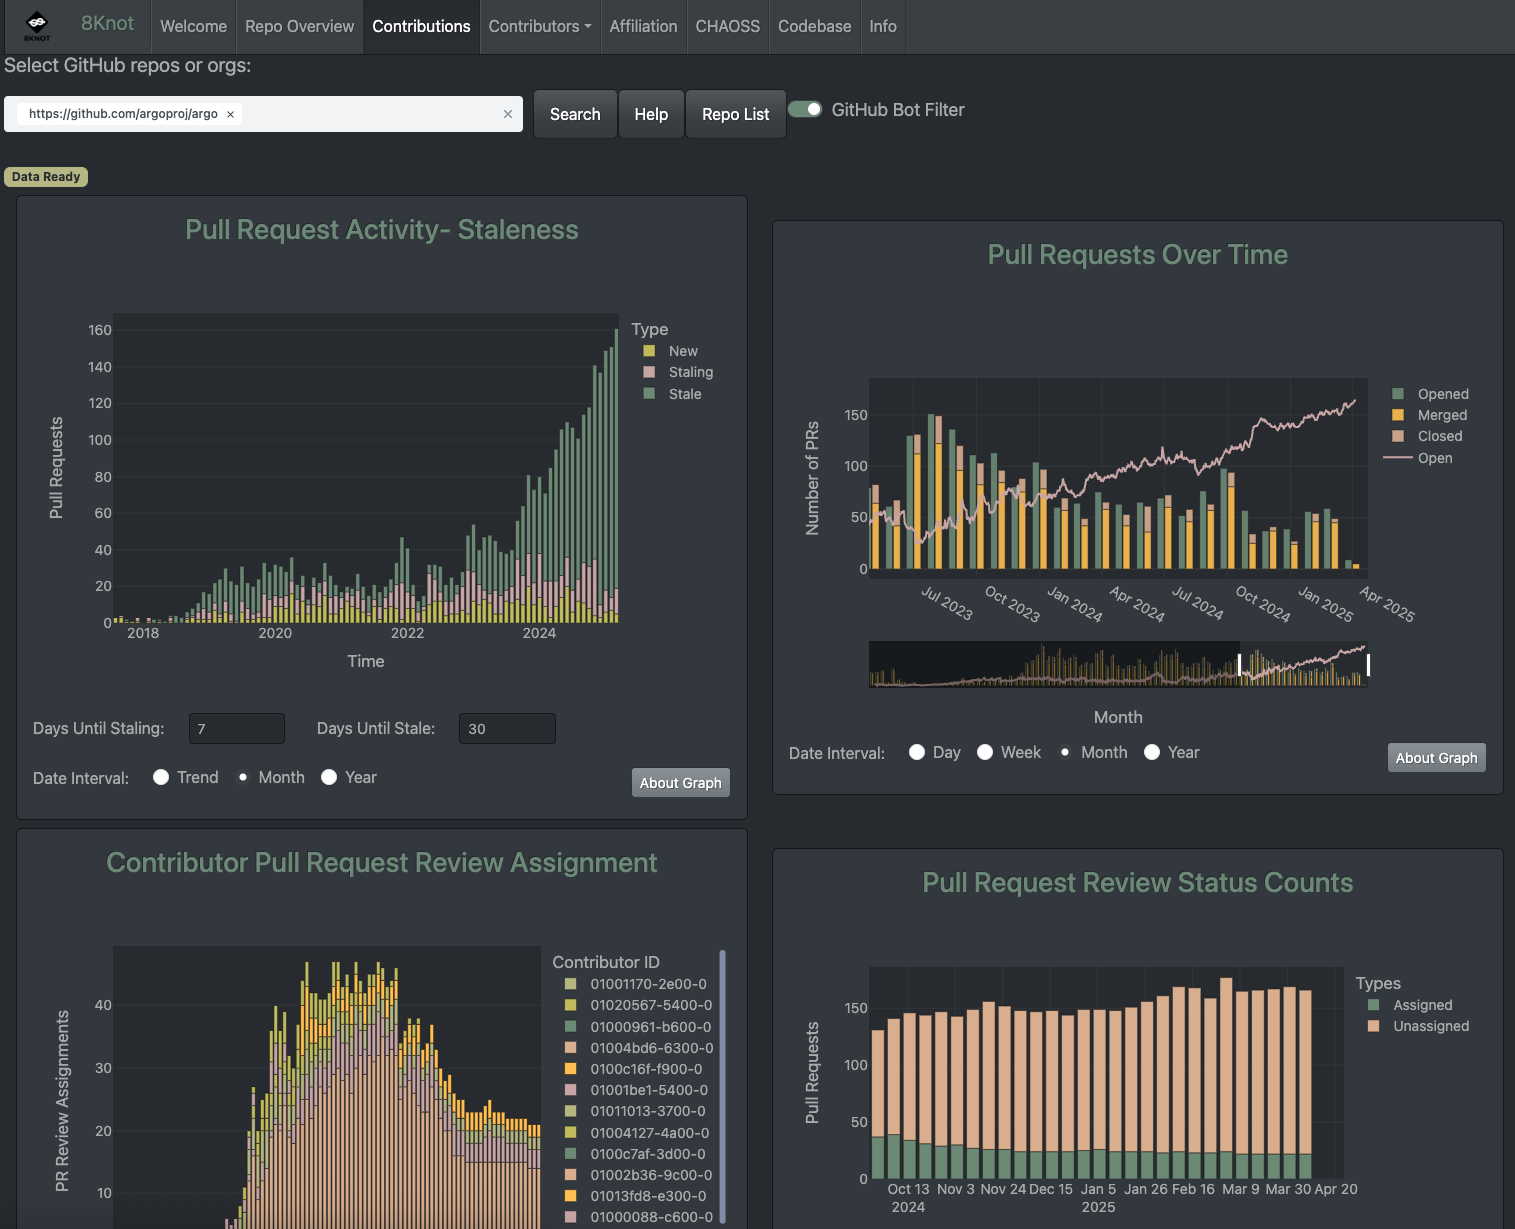
\includegraphics[width=0.9\textwidth]{Figures/augur-8knot.png}
    \caption{Analyse des Projektes Argo mittels Augur \& 8Knot \parencite{noauthor_metrixchaossio_nodate} \parencite{noauthor_argoprojargo-workflows_2025}}
    \label{fig:augur-8knot}
\end{figure}

\newpage


\section{Aufgabenstellung}
Produktivitätsmetriken sollen aus Git-Repositories gewonnen werden. Aus den Daten der Repositories sollen aussagekräftige Kennzahlen für die Softwareentwicklung abgeleitet werden. Dies soll durch eine Literaturrecherche bestehender Metriken und die Entwicklung von Analysealgorithmen erfolgen.
Die offizielle Aufgabenstellung, gestellt von Michael Wahler, befindet sich im Anhang \secref{sec:OffAufgabenstellung}.

\section{Forschungsfragen und Zielsetzung}
\label{sec:Zielsetzung}

Ziel dieser Arbeit ist es, Pull Requests aus Projekten zu untersuchen und deren Eigenschaften hinsichtlich verschiedener Einflussfaktoren zu analysieren. Dabei stehen folgende Forschungsfragen im Vordergrund:

\forschungsfrage{forschungsfrage1}{
Besteht ein Zusammenhang zwischen der Latency eines Pull Requests (Zeit bis zum Merge oder Schliessung) und dem Churn (Anzahl geänderter Codezeilen) des jeweiligen Pull Requests?
}

\forschungsfrage{forschungsfrage2}{
Können die Schliessungsgründe der PRs in den Projekten ermittelt und klassifiziert werden?
}

\forschungsfrage{forschungsfrage3}{
Besteht ein Zusammenhang zwischen dem Zeitpunkt im Projektverlauf und der Review-Dauer von Pull Requests?}


\forschungsfrage{forschungsfrage4}{
Lassen sich Patterns der Zusammenarbeit im Team erkennen, hinsichtlich der Tage, an denen die Studierenden an den Projekten arbeiten?
}

\forschungsfrage{forschungsfrage5}{
Welche Unterschiede zeigen sich in der Nutzung von Pull Requests zwischen Teilzeit- und Vollzeitstudierenden hinsichtlich Anzahl, Umfang und Dauer?
}

\forschungsfrage{forschungsfrage6}{
Welche Unterschiede zeigen sich in den Repository Metriken zwischen den Studentenprojekten und professionellen Github Organisationen?
}

\section{Übersicht der Arbeit}
Im \autoref{Chapter2} \textit{\nameref{Chapter2}} wird das theoretische Wissen vermittelt, welches für das Verständnis dieser Arbeit notwendig ist. Dabei wird auf  Git / GitHub spezifische Methodiken eingegangen, die untersuchten Projekte erläutert und das als Grundlage dienende Tool GitGauge erklärt.

Das \autoref{Chapter3} \textit{\nameref{Chapter3}} beschreibt die Methodik der Arbeit. Es erläutert die Vorgehensweise und beschreibt die notwendigen Metriken zur Klärung der Forschungsfragen. Des Weiteren wird die Datengrundlage aufgezeigt.


Die Ergebnisse werden im \autoref{Chapter4} \textit{\nameref{Chapter4}} dargelegt. Dabei wird auf die spezifischen Forschungsfragen eingegangen und die Analysen zur Beantwortung der Fragen dargestellt. Zusätzlich wird die Erweiterung an der GitGauge-Applikation demonstriert.

Zum Schluss folgt das \autoref{Chapter5} \textit{\nameref{Chapter5}}, in dem noch einmal auf die Forschungsfragen und deren Ergebnisse eingegangen und diese bewertet werden. Ausserdem werden mögliche Erweiterungen aufgezeigt.





